% !TeX document-id = {18c02271-a93d-4ab8-912f-0663088623f3}
%%%%%%%%%%%%%%%%%%%%%%%%%%%%%%%%%%%%%%%%%
% LaTeX Advanced Presentation
%
% Author:
% Alexander Phi. Goetz
% License:
% CC BY-NC-SA 3.0 (http://creativecommons.org/licenses/by-nc-sa/3.0/)
%
%%%%%%%%%%%%%%%%%%%%%%%%%%%%%%%%%%%%%%%%%

%-------------------------------------------------------------------------------
%     PACKAGES AND THEMES
%-------------------------------------------------------------------------------
% !TeX TXS-program:compile = txs:///xelatex/[--shell-escape]
\documentclass[14pt,aspectratio=169]{beamer}
%\documentclass[14pt,aspectratio=169,handout]{beamer}
%\usepackage{pgfpages}
%\pgfpagesuselayout{4 on 1}[a4paper,landscape,border shrink=5mm]

\usepackage[ngerman]{babel}
\usepackage{lipsum}


\setbeameroption{hide notes}

\mode<presentation> {
    %\usetheme[progressbar]{Phictional} % Ab 36 Folien gibts nen Arithmetic overflow ¯\_(ツ)\_/¯
    \usetheme[]{Phictional}
}

%% Linksammlung

% Math-mode Cheat Sheet
\newcommand{\heinkenCheat}{https://www.caam.rice.edu/\~heinken/latex/symbols.pdf}
\newcommand{\fontcalatogue}{https://tug.org/FontCatalogue/}
\newcommand{\ctanFontAwesome}{https://www.ctan.org/pkg/fontawesome5}

% Feedbacklink
\newcommand{\linkMaterial}{https://phictional.de/tutor/LaTeX/}
\newcommand{\linkFeedback}{https://phictional.de/tutor/feedback}



% Hello command for Section 'Commands'
\newcommand{\hello}[1][Phi]{Hallo #1, wie geht's so?}

% Environments
\newenvironment{para}[1]{
    \begin{minipage}{1.5em}
        \rotatebox{90}{\textsc{#1}}
    \end{minipage}\begin{minipage}{\linewidth}
}{
    \end{minipage}\smallskip
}

\newcounter{joke}
\newenvironment{joke}{
    \refstepcounter{joke}
    \noindent\colorbox{gray!50!white}{
        \textbf{Witz~\thejoke}
    } \\[.5em]
}{\medskip}


%% Aufgaben
% Aufgabe 1
\newcommand{\bbR}{\mathbb{R}}
\newcommand{\bbZ}{\mathbb{Z}}
\newcommand{\bbQ}{\mathbb{Q}}
\newcommand{\bbN}{\mathbb{N}}
\newcommand{\bbC}{\mathbb{C}}

% Aufgabe 2
\newcommand{\aufgabe}[2]{
    \section*{Aufgabe #1\hfill\small\textcolor{gray}{(#2 Punkte)}}
}

% Aufgabe 3
\newenvironment{loesung}[1][Lösung]{
    \medskip
    \noindent\textbf{#1}: 
    
    \medskip\noindent
}{\\\smallskip}


%% FONTS
% https://tug.org/FontCatalogue/comicneue/
\newcommand{\comicneue}{\fontfamily{ComicNeue-TLF}\selectfont}
\DeclareTextFontCommand{\textcn}{\comicneue}






%-------------------------------------------------------------------------------
%     TITLE PAGE
%-------------------------------------------------------------------------------

% short title for footline and long title for title page
\title[\LaTeX\ Advanced]{\uppercase{Weiterführendes \LaTeX}} 
\subtitle{\uppercase{Eigene Environments bis hin zu eigenen Packages}}

\date[14.04.22]{\itshape 14. April 2022} % date

% short name for footline and long name for title page
\author[\textbf{Phi}]{Alexander \emph{Phi} Goetz 
        \scriptsize | \texttt{info@phictional.de}}

% short institute for footline and long institute for title page
\institute[FSI]{Fachschaft Informatik Uni Tübingen \scriptsize \\  
                \url{fsi@fsi.uni-tuebingen.de}} 


\begin{document}

\titleframe


\frame{\textbf{\emph{\Large Disclaimer}}: \\ 
        Dieser Workshop baut direkt auf dem Workshop von heute Vormittag auf!}


\begin{frame}
	\frametitle{Inhalte}
    \begin{columns}
        \column{.7\textwidth}
        \tableofcontents
        
        \column{.3\textwidth}
        \centering
        {\faFileDownload\Large Material}
        \material[height=.7\textwidth]{\linkMaterial}
    \end{columns}
\end{frame}


%-------------------------------------------------------------------------------
%     PRESENTATION SLIDES
%-------------------------------------------------------------------------------

%%%%%%%%%%%%%%%%%%%%%%%%%%
%%      Commands        %%
%%%%%%%%%%%%%%%%%%%%%%%%%%

\section{Commands}
\begin{frame}
    \sectionpage
    \vspace{.5em}
    \large\faFolderOpen \normalsize \mintinline{sh}{live/01_commands_and_environments/} 
\end{frame}

\begin{frame}{\insertsection}
    \begin{columns}
        \column{.7\textwidth}
        Commands ohne Argument:
        \[\mintinline{tex}{\leq} \quad\Rightarrow\quad \leq\]
        
        Commands \textbf{mit} \textcolor{lightgray}{[optionalen]} Argumenten:
        
        \begin{align*}
            &\mintinline{tex}{\sqrt{4}}    &&\Rightarrow\quad \sqrt{4} \\
            &\mintinline{tex}{\sqrt[3]{4}} &&\Rightarrow\quad \sqrt[3]{4}
        \end{align*}
        
        
        \column{.3\textwidth}
        \material[height=.7\textwidth]{\heinkenCheat}
    \end{columns}
\end{frame}

% \newcommand
\begin{frame}
    \frametitle{\insertsection \small\quad \mintinline{tex}{\newcommand}}
    \label{newc}
    \begin{Definition}
        
        \vspace{1em}
        \mint[linenos,xleftmargin=2em]{tex}{\newcommand{name}[n][defaultFirst]{body}}
        \vspace{1em}
        
        \setbeamercolor{itemize item}{fg=eigengrau}
        \begin{itemize}%[<+->]
            \item \textbf{\texttt{name}}: Name des Befehls
            \item \textbf{\texttt{n}}: Anzahl von Parametern
            \item \textbf{\texttt{defaultFirst}}: Standartwert für ersten Parameter
            \item \textbf{\texttt{body}}: Hier werden Parameter mittels \textbf{\texttt{\#x}}, 
                                           $\textbf{\texttt{x}} \in \{1,...,n\}$ verwendet
        \end{itemize}
    \end{Definition}  
\end{frame}

\begin{frame}[fragile]
    \frametitle{\insertsection \small\quad \mintinline{tex}{\newcommand}}
    
    \begin{Beispiel}[\mintinline{tex}{\hello}]
        \begin{minted}[linenos, xleftmargin=2em,fontsize=\small]{tex}
\newcommand{\hello}[1][Phi]{Hallo #1, wie geht's so?}
            
\hello \\
\hello[Jules]
        \end{minted}
    \end{Beispiel}
   
    \pause
   
    \begin{exampleblock}{Ausgabe}
        \hello\\
        \hello[Jules]
    \end{exampleblock}
\end{frame}


% \renewcommand
\begin{frame}
    \frametitle{\insertsection \small\quad \mintinline{tex}{\renewcommand}}
    \label{renewc}
    \begin{Definition}
    99\% identisch zu \mintinline{tex}{\newcommand}$^\text{\ref{newc}}$
    
    \vspace{1em}
    \mint[linenos,xleftmargin=2em]{tex}{\renewcommand{name}[n][defaultFirst]{body}}
    \vspace{1em}
    
    \setbeamercolor{itemize item}{fg=eigengrau}
    \begin{itemize}%[<+->]
        \item \textbf{\texttt{name}}: Name des Befehls
        \item \textbf{\texttt{n}}: Anzahl von Parametern
        \item \textbf{\texttt{defaultFirst}}: Standartwert für ersten Parameter
        \item \textbf{\texttt{body}}: 
                Hier werden Parameter mittels \textbf{\texttt{\#x}}, 
                $\textbf{\texttt{x}} \in \{1,...,n\}$ verwendet
    \end{itemize}
\end{Definition}  
\end{frame}

\begin{frame}[fragile]
    \frametitle{\insertsection \small\quad \mintinline{tex}{\renewcommand}}
    
    \begin{Beispiel}[\mintinline{tex}{\square}]
        \begin{minted}[linenos, xleftmargin=2em,fontsize=\small]{tex}
$\Box\square$

\renewcommand{\square}{^2}
$\Box\square$
        \end{minted}
    
    \note{\mintinline{tex}{\square} ist standartmäßig eine \colorbox{accent2}{$\Box$}, wird aber mit
          \texttt{renewcommand} zu einer hochgestellten zwei \colorbox{accent2}{$^2$}.\\
          Der Befehl kann vorher wie nacher nur im \emph{Mathe-Modus} verwendet werden.}
    
    \end{Beispiel}
    
    \pause
    
    \begin{exampleblock}{Ausgabe}
        $\Box\square$
        
        $\Box^2$
    \end{exampleblock}
\end{frame}


%%%%%%%%%%%%%%%%%%%%%%%%%%%%%%
%%      Environments        %%
%%%%%%%%%%%%%%%%%%%%%%%%%%%%%%

\section{Environments}
\begin{frame}
    \sectionpage
    \vspace{.5em}
    \large\faFolderOpen \normalsize \mintinline{sh}{live/01_commands_and_environments/} 
\end{frame}

\begin{frame}[fragile]{\insertsection}
    
    Die bekannte Umgebung \textbf{\texttt{table}}: \vspace{1em}
    
    \begin{columns}
        \column{.5\textwidth}
        
        \begin{minted}[linenos,xleftmargin=2em,fontsize=\footnotesize]{tex}
\begin{table}
    \begin{tabular}{l|c}
        Workshop & Teilnehmer \\
        \hline
        Bash     & 20 \\
        Git      & 20 \\
        Python   & 20 \\
        LaTeX    & 20 \\
        \dots    
    \end{tabular}
    \caption{Teilnehmer}
\end{table}
        \end{minted}
        
        \column{.5\textwidth}
        
        \begin{table}
            \begin{tabular}{l|c}
                Workshop & Teilnehmer \\
                \hline
                Bash     & 20 \\
                Git      & 20 \\
                Python   & 20 \\
                LaTeX    & 20 \\
                \dots    
            \end{tabular}
            \caption{Teilnehmer}
        \end{table}
    \end{columns}
    

    \note{}
\end{frame}

\begin{frame}
    \frametitle{\insertsection \small\quad \mintinline{tex}{\newenvironment}}
    \label{newe}
    \begin{Definition}
        \mint[linenos,xleftmargin=2em]{tex}{\newenvironment{name}[n][defaultFirst]{before}{after}}
        \vspace{.5em}
        
        \setbeamercolor{itemize item}{fg=eigengrau}
        \begin{itemize}%[<+->]
            \item \textbf{\texttt{name}}:   Name des Befehls
            \item \textbf{\texttt{n}}:      Anzahl von Parametern
            \item \textbf{\texttt{defaultFirst}}: Standartwert für ersten Parameter
            \item \textbf{\texttt{before}}: 
                    Der Code der \textit{vor} dem Inhalt kommt
            \item \textbf{\texttt{after}}: 
                    Der Code der \textit{nach} dem Inhalt kommt
        \end{itemize}
        \vspace{.5em}
    
        Zwischen \textbf{\texttt{before}} und \textbf{\texttt{after}} landet der
        Code, der zwischen \\ 
        \mintinline{tex}{\begin{name}} und \mintinline{tex}{\end{name}} geschrieben wird.
    \end{Definition}  
\end{frame}

\begin{frame}[fragile]
    \frametitle{\insertsection \small\quad \mintinline{tex}{\newenvironment} mit Nummerierung}
    \label{newe}
    \begin{Definition}
        \begin{minted}[linenos,xleftmargin=2em,fontsize=\small]{tex}
\newcounter{name}         % Zähler anlegen
\newenvironment{name}[n][defaultFirst]{
    \refstepcounter{name} % Referenzieren zum Inkrementieren
    \thename              % Zahl abrufen
    before
}{after}
        \end{minted}
    
        
    \end{Definition}  

    Funktioniert so auch in normalen \emph{Commands}. Siehe \mintinline{tex}{\section}.
\end{frame}

\begin{frame}[fragile]
    \frametitle{\insertsection \small\quad \mintinline{tex}{\newenvironment}}
    
    \begin{Beispiel}[\mintinline{tex}{\newenvironment}]
        \begin{minted}[linenos, xleftmargin=2em,fontsize=\small]{tex}
\newenvironment{para}[1]{
    \begin{minipage}{1.5em}
        \rotatebox{90}{\textsc{#1}}
    \end{minipage}\begin{minipage}{\linewidth}
}{
    \end{minipage}\smallskip
}
        \end{minted}
        
        \note{}
        
    \end{Beispiel}
    
    \vspace{-1.5em}
    
    \begin{overprint}
        \onslide<1>\begin{itemize}
            \vspace{.5em}
            \item \mintinline{tex}{minipage} ermöglicht es horizontal ''Boxen'' anzulegen.\\
            \item \mintinline{tex}{\rotatebox[Winkel]{Inhalt}} dreht den Inhalt um den angegebenen Winkel.
        \end{itemize}
        
        \onslide<2>\begin{exampleblock}{Ausgabe}
            \begin{para}{Test}
                Hier steht ein bisschen Fülltext.
            \end{para}
        \end{exampleblock}
    \end{overprint}
\end{frame}


\begin{frame}[fragile]
    \frametitle{\insertsection \small\quad \mintinline{tex}{\newenvironment} mit Nummerierung}
    
    \begin{columns}[t]
        \column{.5\linewidth}
        \begin{Beispiel}[\mintinline{tex}{\newenvironment}]
            \begin{minted}[linenos, xleftmargin=2em,fontsize=\small]{tex}
\newcounter{joke}
\newenvironment{joke}{
    \refstepcounter{joke}
    \noindent
    \colorbox{gray!50!white}{
        \textbf{Witz~\thejoke}
    } \\[.5em]
}{\medskip}
            \end{minted}           
        \end{Beispiel}
        
        \column{.01\linewidth}
        
        \column{.45\linewidth}
        \begin{exampleblock}{Ausgabe}
            \begin{joke}
                Wie nennt man eine Zauberin in der Wüste? \\
                \textbf{Sand Witch!}
            \end{joke}
        \end{exampleblock}
        
    \end{columns}
\end{frame}

\begin{frame}{\insertsection \small\quad \mintinline{tex}{\renewenvironment}}
    \begin{Definition}
         \mint{tex}{\renewenvironment{name}[n][defaultFirst]{before}{after}}
    \end{Definition}
    
    Auch hier gibt es wieder ein \mintinline{tex}{\renewenvironment}. Es verhält
    sich genauso wie \mintinline{tex}{\newenvironment} und überschreibt die vorher
    definierte/importierte Umgebung.
\end{frame}


%%======================%%
%%      Aufgaben        %%
%%======================%%

\section*{Aufgaben}
\sectionframe

\begin{frame}{\insertsection}
    Es gibt den Befehl \mintinline{tex}{\mathbb{}} für den Mathe-Modus.
    \colorbox{accent2!50!white}{$ \mintinline{tex}{\mathbb{R}} \Rightarrow \mathbb{R} $}
    
    \begin{alertblock}{Aufgabe \aufgabennummer:\quad Zahlenräume}
        Schreibe 
            \[ \bbN \subset \bbZ \subset \bbQ \subset \bbR \subset \bbC \]
        mittels Custom Commands nach dem Muster
            \[ \mintinline{tex}{\bbR} \Rightarrow \bbR
                        \quad\text{oder}\quad
               \mintinline{tex}{\bb{R}} \Rightarrow \bbR \]
    \end{alertblock}
\end{frame}

\begin{frame}{\insertsection}
    \begin{alertblock}{Aufgabe \aufgabennummer:\quad Aufgaben-Section mit Punkten}
        Ziemlich was der Titel sagt. Entwerfe einen Befehl 
        \mintinline[]{tex}{\aufgabe}, der \textbf{zwei}
        Argumente erwartet:
        
        \setbeamercolor{itemize item}{fg=eigengrau}
        \begin{itemize}
            \item Nummer der Aufgabe
            \item Punkte für die Aufgabe
        \end{itemize}
        Hilfreiche Befehle sind \mintinline{tex}{\section*} und \mintinline{tex}{\hfill}.\\
        Optional sind \mintinline{tex}{\small} und 
        \mintinline{tex}{\textcolor{color}{text}}.
        
        \begin{figure}
            \includegraphics[width=.8\linewidth]{pictures/aufgabe\_2.png}
        \end{figure}
    \end{alertblock}
\end{frame}

\begin{frame}{\insertsection}
    \begin{alertblock}{Aufgabe \aufgabennummer:\quad Lösungs-Umgebung}
        
        \begin{columns}
            \column{.6\linewidth}
            
            Entwerfe eine Umgebung \mintinline{tex}{loesung}, die den Text 
            ''\textbf{Lösung}:'' als Präfix besitzt.\\
            Der Präfix ist der einzige und optionale Parameter.\\[.5em]
            
            Hilfreiche Befehle:
            \setbeamercolor{itemize item}{fg=eigengrau}
            \begin{itemize}
                \item \mintinline{tex}{\medskip} vertikaler Lücke
                \item \mintinline{tex}{\noindent} keine Einrückung
                \item \mintinline{tex}{\textbf{}} Fett geschrieben
            \end{itemize}
                    
            \column{.3\linewidth}
            
            \begin{loesung}
                So sieht die \mintinline{tex}{loesung}-Umgebung in Verwendung aus.
            \end{loesung}
                        
        \end{columns}        
    \end{alertblock}
\end{frame}


%%%%%%%%%%%%%%%%%%%%%%%
%%      Fonts        %%
%%%%%%%%%%%%%%%%%%%%%%%

\section{Fonts}
\begin{frame}
    \sectionpage
    \vspace{.5em}
    \large \faFolderOpen \mintinline{sh}{live/02_fonts/} 
\end{frame}


\subsection{Font Styles}

\begin{frame}{\insertsubsection}
    \begin{figure}
        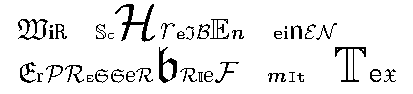
\includegraphics[width=\textwidth]{pictures/erpresserbrief.pdf}
        \caption{Mit Font Styles und Sizes freidrehen}
    \end{figure}
\end{frame}


\begin{frame}[fragile]{\insertsubsection \quad\small Größe}
    \begin{table}
        \begin{tabular}{c|c|c|c|c}
            \mintinline{tex}{\tiny}  & \mintinline{tex}{\scriptsize} 
            & \mintinline{tex}{\footnotesize} & \mintinline{tex}{\small} 
                & \mintinline{tex}{\normalsize} \\
            \hline
            {\tiny Text}             & {\scriptsize Text}
            & {\footnotesize Text}            & {\small Text}
                & {\normalsize Text}            \\
            \hline\hline
            \mintinline{tex}{\large} & \mintinline{tex}{\Large} 
            & \mintinline{tex}{\LARGE}        & \mintinline{tex}{\huge} 
                & \mintinline{tex}{\Huge} \\
            \hline
            {\large Text}            & {\Large Text}
            & {\LARGE Text}                   & {\huge Text}            
                & {\Huge Text} 
        \end{tabular}
        \caption{Font Sizes in Tex}
    \end{table}

    \vspace{-0.5em}
    
    \begin{Beispiel}[Verwendung von \mintinline{tex}{\tiny}]
        \begin{figure}
            \vspace{-0.5em}
            \begin{minted}[linenos,xleftmargin=2em,fontsize=\small]{tex}
{\tiny So werden die Schriftgrößen verwendet!}
            \end{minted}
            \vspace{.5em}
            {\tiny So werden die Schriftgrößen verwendet!}
        \end{figure}
        \vspace{-0.5em}
    \end{Beispiel}
\end{frame}


\begin{frame}{\insertsubsection \quad\small Stil}
    \begin{table}
        \begin{tabular}{l|c||l|c}
            %\hline
            Mathe Text Style & & Text Style & \\
            \hline
            \mintinline{tex}{$\mathcal{A}$}  & ~~$\mathcal{A}$~~   
            & \mintinline{tex}{\textbf{Text}}  & ~~\textbf{Text}~~  \\
            \mintinline{tex}{$\mathbb{A}$}   & ~~$\mathbb{A}$~~    
            & \mintinline{tex}{\textit{Text}}  & ~~\textit{Text}~~  \\
            \mintinline{tex}{$\mathfrak{A}$} & ~~$\mathfrak{A}$~~  
            & \mintinline{tex}{\texttt{Text}}  & ~~\texttt{Text}~~  \\
            \mintinline{tex}{$\mathsf{A}$}   & ~~$\mathsf{A}$~~    
            & \mintinline{tex}{\textsf{Text}}  & ~~\textsf{Text}~~ \\
            \mintinline{tex}{$\mathbf{A}$}   & ~~$\mathbf{A}$~~    
            & \mintinline{tex}{\textrm{Text}}  & ~~\textrm{Text}~~  \\
            %\hline
        \end{tabular}
        \caption{Font Styles für Text im Mathe-Modus, sowie den Text-Modus}
    \end{table}
    \vspace{-1em}
    \begin{table}
        \begin{tabular}{c|c}
            \mintinline{tex}{\uppercase{LaTeX}} & \mintinline{tex}{\lowercase{LaTeX}} \\
            \hline
            \uppercase{LaTeX}                   & \lowercase{LaTeX}
        \end{tabular}
        \caption{Alles groß-/kleinschreiben ist kein Problem}
    \end{table}
\end{frame}


\subsection{Andere Fonts}

\begin{frame}{\insertsubsection}
    \Large\emph{\faQuoteLeft}
    Schriftarten, die nicht ,,häufig'' vorkommen, \\ 
    \textcolor{white}{\faQuoteLeft} sind verdammt nervig. 
\end{frame}

\begin{frame}[fragile]
    \frametitle{\insertsubsection \small\quad Dokumenten-Schriftart}
    \begin{columns}
        \column{.7\linewidth}
        
        \begin{overprint}
            \onslide<1>
            \textbf{MiKTeX}, \textbf{TeX Live} werden mit einer 
            Auswahl von Schriftarten ausgeliefert.
            \begin{figure}
                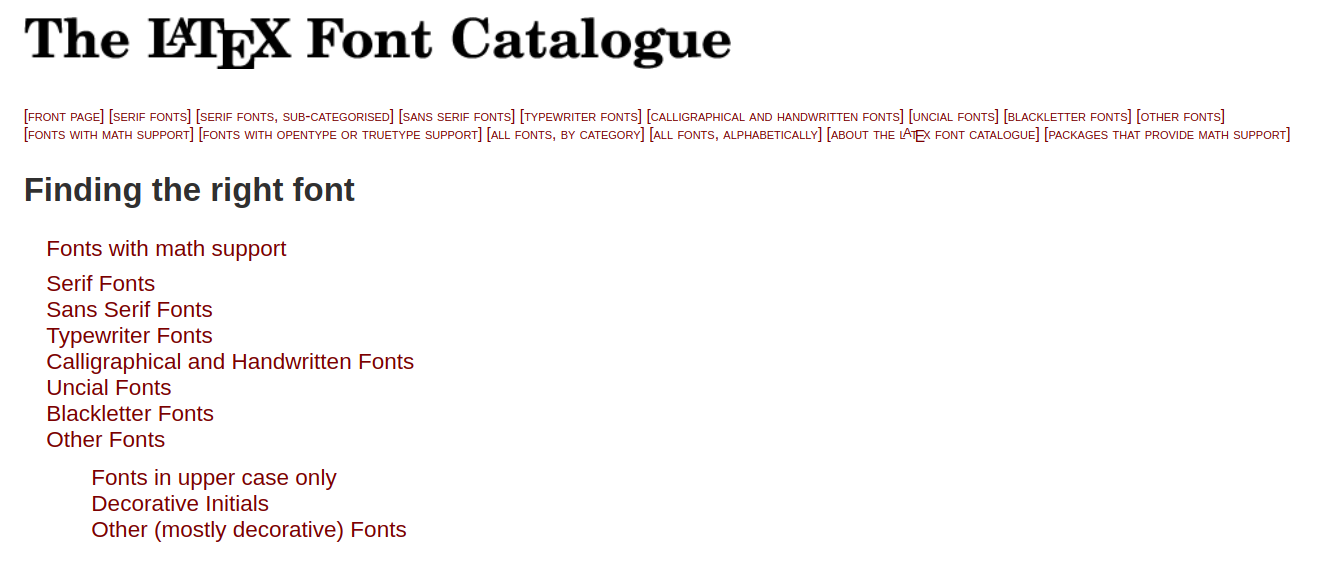
\includegraphics[width=.9\textwidth]{pictures/font_catalogue.png}
            \end{figure}
        
            \onslide<2>
            \begin{Definition}
                \begin{minted}[linenos,xleftmargin=2em]{tex}
\usepackage[T1]{fontenc}
\usepackage{fontname}
                \end{minted}
                
                Der Standart-Weg um \textbf{dokumentenweit} Fonts einzustellen
                (unter \textit{pdf(La)TeX} und \textit{MiKTeX}). \\[.5em]                
                \textit{Xe(La)TeX}/\textit{Lua(La)TeX} verwenden das Package
                \mintinline{tex}{fontspec} und sind iA. besser im Umgang mit
                Schriftarten.
            \end{Definition}
        
            \onslide<3>
            \begin{Beispiel}[Comic Sans-ish]
                \begin{minted}[linenos,xleftmargin=2em]{tex}
\usepackage[T1]{fontenc}
\usepackage[default]{comicneue}
                \end{minted}
                
                \begin{figure}
                    
\includegraphics[width=.8\textwidth]{pictures/comicneue.pdf}
                    \caption{Die Schriftart in Verwendung}
                \end{figure}
            \end{Beispiel}
                        
        \end{overprint}
                
        \column{.3\linewidth}
        \material[height=.7\linewidth]{\fontcalatogue}        
    \end{columns}
\end{frame}

\begin{frame}[fragile]{\insertsubsection \small\quad Inline Schriftart}
    In \textbf{Word}\faFileWord kann man einzelne Textschnipsel in verschiedenen 
    Schriftarten schreiben. Geht das in TeX auch? \quad\textbf{Ja, aber umständlicher.}
    
    \begin{Beispiel}[Inline]
        \begin{minted}[linenos,xleftmargin=2em,fontsize=\small]{tex}
Hier steht was. 
{\fontfamily{ComicNeue-TLF}\selectfont Hier Comic Neue.} 
Hier wieder nicht.
        \end{minted}
        
        \begin{figure}
            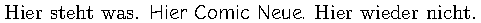
\includegraphics[width=.8\linewidth]{pictures/comicneue_inline.pdf}
            \caption{Umständliches Inline}
        \end{figure}
    \end{Beispiel}
\end{frame}


\begin{frame}[fragile]{\insertsubsection \small\quad Inline Schriftart}
    
    \begin{Definition}
        \begin{minted}[linenos,xleftmargin=2em,fontsize=\small]{tex}
\newcommand{\comicneue}{\fontfamily{ComicNeue-TLF}\selectfont}
\DeclareTextFontCommand{\textcn}{\comicneue}
        \end{minted}
    \end{Definition}
    
    \begin{overprint}
        \onslide<1>
        \mintinline{tex}{\textcn} wird dann so verwendet wie \mintinline{tex}{\textbf}, 
        \mintinline{tex}{\textrm}, \mintinline{tex}{\textsc}, ...
                
        \vspace{.5em}
        
        Wie kommen wir überhaupt auf \textbf{\texttt{ComicNeue-TLF}}? 
        \begin{enumerate}
            \item Gewünschte Schriftart als Standart setzen 
            (\mintinline{tex}{\usepackage{...}})
            \item Im Text \mintinline{tex}{\familydefault}
            \item Dieser String ist die gesuchte \mintinline{tex}{fontfamily}
        \end{enumerate}
        
                
        \onslide<2>
        \vspace{-1em}
        
        \begin{Beispiel}[\mintinline{tex}{\comicneue}\ /\ \mintinline{tex}{\textcn}]
            \begin{minted}[linenos,xleftmargin=2em,fontsize=\small]{tex}
{\comicneue Hier steht etwas auf diese Weise} \\
\textcn{Hier steht etwas auf die andere Weise}
            \end{minted}
            \begin{figure}
                \vspace{-.5em}
                
                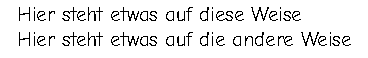
\includegraphics[width=.6\linewidth]{pictures/comicneue_commands.pdf}
                \vspace{-1em}
                
                \caption{Nützlicheres Inline}
                \vspace{-1em}
            \end{figure}
        \end{Beispiel}
    \end{overprint}
\end{frame}

%%======================%%
%%      Aufgaben        %%
%%======================%%

\section*{Aufgaben}
\sectionframe

% TODO: fontawesome

\begin{frame}{\insertsection}
    \begin{alertblock}{Aufgabe \aufgabennummer: \quad Neue Monospaced Schriftart}
        Suche dir im \textbf{\LaTeX  Font Catalogue}\footnote{\fontcalatogue} eine neue
        Typewriter-Font aus, die die \textbf{Computer Modern} Monospace Schriftart
        ersetzt. \\
        \textcolor{gray}{(Ich empfehle \textbf{Fira Mono} oder \textbf{DejaVu Sans Mono})}
        
        \begin{table}
            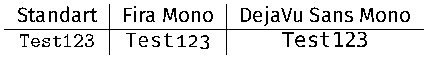
\includegraphics[width=.6\textwidth]{pictures/monospaced.pdf}
            \caption{Vergleich der Schriftarten}
        \end{table}
        
        % https://tug.org/FontCatalogue/firamono/
        % https://tug.org/FontCatalogue/dejavumono/
    \end{alertblock}
\end{frame}


\begin{frame}{Aufgaben}
    \begin{columns}
        \column{.7\textwidth}
            
        \begin{alertblock}{Aufgabe \aufgabennummer: \quad Awesome Fonts \small\faGrinHearts[regular]}
            Neben den normalen Schriftarten gibts auch andere witzige Dinge.\\[1em]        
            Deine Aufgabe ist es folgende Sequenz von Symbolen anzugeben:
            
            \begin{figure}
                
\includegraphics[width=.9\textwidth]{pictures/awesome.pdf}
                \caption{Die Symbolsequenz}
            \end{figure}
        
            \vspace{-1em}
        \end{alertblock}
            
        \column{.3\textwidth}
            
        \centering
        \large Startpunkt
        \material[height=.7\textwidth]{\ctanFontAwesome}
    \end{columns}
\end{frame}
%% Aufgaben

% https://www.ctan.org/pkg/fontawesome5
% https://ftp.fau.de/ctan/fonts/fontawesome5/doc/fontawesome5.pdf
%\usepackage{fontawesome5}

%%%%%%%%%%%%%%%%%%%%%%%%%%%
%%      Packgages        %%
%%%%%%%%%%%%%%%%%%%%%%%%%%%

\section{Packages}
\begin{frame}
    \sectionpage
    \vspace{.5em}
    \large \faFolderOpen \mintinline{sh}{live/03_packages/}   
\end{frame}


\begin{frame}{\insertsection \quad\small Motivation}
	
	\textbf{Warum der Spaß?}
	
    \begin{itemize}
        \item Die Präambel läuft über / ist zu lang.
        \item Viele Dokumente mit der selben / ähnlichen Präambel (Übungsblätter)
        \item Befehle mit anderen teilen
    \end{itemize}
    
    \pause
    
    \begin{exampleblock}{Idee}
    	Präambel in eine \mintinline{sh}{settings.tex} packen. \\
    	\mintinline{tex}{%==================================================================
% 		Preface in its own file
%==================================================================

\usepackage[utf8]{inputenc}
\usepackage[ngerman]{babel}
\usepackage{amsmath}
\usepackage{amssymb}
\usepackage{fancyhdr}
\usepackage{color}
\usepackage{graphicx}
\usepackage{lastpage}
\usepackage{listings}
\usepackage{tikz}
\usepackage{pdflscape}
\usepackage{subfigure}
\usepackage{float}
\usepackage{polynom}
\usepackage{hyperref}
\usepackage{tabularx}
\usepackage{forloop}
\usepackage{geometry}
\usepackage{listings}
\usepackage{fancybox}
\usepackage{tikz}
\usepackage{algpseudocode,algorithm,algorithmicx}

%------------------------------------------------------------------------------
%     START: Our Commands & Environments
%------------------------------------------------------------------------------
\usepackage{lipsum} % Für Fülltext

%% Commands
% Slide 7
\newcommand{\hello}[1][Phi]{Hallo #1, wie geht's so?}

% Slide 9
%\renewcommand{\square}{^2}


%% Environments
% Slide 12
\newenvironment{para}[1]{
	\begin{minipage}{1.5em}
		\rotatebox{90}{\textsc{#1}}
	\end{minipage}\begin{minipage}{\linewidth}
	}{\end{minipage}\smallskip}

% Slide 13
\newcounter{joke}
\newenvironment{joke}{
	\refstepcounter{joke}
	\noindent
	\colorbox{gray!50!white}{
		\textbf{Witz~\thejoke}
	} \\[.5em]
}{\medskip}


%% Aufgaben
% Aufgabe 1: Zahlenräume
\newcommand{\bbR}{\mathbb{R}}
\newcommand{\bbZ}{\mathbb{Z}}
\newcommand{\bbQ}{\mathbb{Q}}
\newcommand{\bbN}{\mathbb{N}}
\newcommand{\bbC}{\mathbb{C}}

% Aufgabe 2: Aufgaben-Section mit Punkten
\newcommand{\aufgabe}[2]{
	\section*{Aufgabe #1\hfill\small\textcolor{gray}{(#2 Punkte)}}
}

% Aufgabe 3: Lösungs-Umgebung
\newenvironment{loesung}[1][Lösung]{
	\medskip
	\noindent\textbf{#1}: 
	
	\medskip\noindent
}{\\\smallskip}


%% Fonts

% Andere "Schriftarten"
% https://tug.org/FontCatalogue/
\usepackage[T1]{fontenc} % Notwendig für so ziemlich jede Schriftart
% \usepackage{fontspec}  % Für Xe(La)TeX und Lua(La)TeX

% Dokumentenweit
% https://tug.org/FontCatalogue/comicneue/
%\usepackage[default]{comicneue}

% Inline
\newcommand{\comicneue}{\fontfamily{ComicNeue-TLF}\selectfont}
\DeclareTextFontCommand{\textcn}{\comicneue}


%% Aufgaben
% Aufgabe 4: Neue Monospaced Schriftart
% https://tug.org/FontCatalogue/firamono/
\usepackage{FiraMono}

% Aufgabe 5: Awesome Fonts
% https://www.ctan.org/pkg/fontawesome5
% https://ftp.fau.de/ctan/fonts/fontawesome5/doc/fontawesome5.pdf
\usepackage{fontawesome5}



%------------------------------------------------------------------------------
%     END: Our Commands & Environments
%------------------------------------------------------------------------------

%Definiere Let-Command für algorithmen
\newcommand*\Let[2]{\State #1 $\gets$ #2}

%Größe der Ränder setzen
\geometry{a4paper,left=3cm, right=3cm, top=3cm, bottom=3cm}

%Kopf- und Fußzeile
\pagestyle {fancy}
\fancyhead[L]{Tutor: \TUTOR}
\fancyhead[C]{\COURSE}
\fancyhead[R]{\today}

\fancyfoot[L]{}
\fancyfoot[C]{}
\fancyfoot[R]{Seite \thepage /\pageref*{LastPage}}

%Formatierung der Überschrift, hier nichts ändern
\def\header#1#2{
	\begin{center}
		{\Large Übungsblatt #1}\\
		{(Abgabetermin #2)}
	\end{center}
}

%Definition der Punktetabelle, hier nichts ändern
\newcounter{punktelistectr}
\newcounter{punkte}
\newcommand{\punkteliste}[2]{%
	\setcounter{punkte}{#2}%
	\addtocounter{punkte}{-#1}%
	\stepcounter{punkte}%<-- also punkte = m-n+1 = Anzahl Spalten[1]
	\begin{center}%
		\begin{tabularx}{\linewidth}[]{@{}*{\thepunkte}{>{\centering\arraybackslash} X|}@{}>{\centering\arraybackslash}X}
			\forloop{punktelistectr}{#1}{\value{punktelistectr} < #2 } %
			{%
				\thepunktelistectr &
			}
			#2 &  $\Sigma$ \\
			\hline
			\forloop{punktelistectr}{#1}{\value{punktelistectr} < #2 } %
			{%
				&
			} &\\
			\forloop{punktelistectr}{#1}{\value{punktelistectr} < #2 } %
			{%
				&
			} &\\
		\end{tabularx}
	\end{center}
}
} anstatt der alten Präambel.
    \end{exampleblock}
\end{frame}


\begin{frame}{Einschub}	
	\begin{exampleblock}{\mintinline{tex}{\input} vs \mintinline{tex}{\include}}
		\begin{columns}[t]
			\column{.5\linewidth}
			\mint[linenos,xleftmargin=2em]{tex}{\input{filename}}
			
			\begin{itemize}
				\item Importiert \texttt{filename.tex}
				\item Als ob Code in aufrufender Datei stehen würde
				\item Befehle verwendbar
			\end{itemize}
			
			\column{.5\linewidth}
			\mint[linenos,xleftmargin=2em]{tex}{\include{filename}}
			
			\begin{itemize}
				\item Importiert \texttt{filename.tex}
				\item In Kompilation eigene Datei
				\item Befehle nicht verwendbar
	       		\item nützlich bei großen Projekten \\
    				  mit Teildokumenten
			\end{itemize}
		\end{columns}
        \vspace{1em}
        
	\end{exampleblock}	
\end{frame}


\begin{frame}[fragile]{\insertsection \quad\small Was ist ein Package?}
    Eine Sammlung von Befehlen und Umgebungen, die in anderen Dokumenten eingesetzt
    werden kann.
    
    \begin{overprint}
        \onslide<1>
        Nicht viel anders zur \mintinline{sh}{settings.tex}-Lösung. Die Unterschiede sind:
        
        \begin{enumerate}
            \item Dateiendung \mintinline{sh}{.sty}
            \item Einbindung mittels \mintinline{tex}{\usepackage{packagename}}
            \item Angabe des ''Headers''
            \begin{minted}[linenos,xleftmargin=2em,fontsize=\small]{tex}
\NeedsTeXFormat{LaTeX2e}
\ProvidesPackage{packagename}[YYYY/MM/dd package description]
            \end{minted}
            \item \mintinline{tex}{\usepackage} {\small\faArrowRight} \mintinline{tex}{\RequirePackage}
        \end{enumerate}
    
        \onslide<2>
        Nicht viel anders zur \mintinline{sh}{settings.tex}-Lösung. Besonderheiten:
        
        \begin{itemize}
            \item \mintinline{tex}{\newcommand} kann weiter verwendet werden
            \item \mintinline{tex}{\renewcommand} kann weiter verwendet werden
            \item \mintinline{tex}{\providecommand} definiert Befehl, falls nicht schon vorher vorhanden
            \item \mintinline{tex}{\CheckCommand} genau wie \mintinline{tex}{\newcommand}, 
                  falls Befehl bereits vorhanden und anders als in \mintinline{tex}{\CheckCommand}
                  definiert gibts \textbf{Error}
        \end{itemize}
    \end{overprint}
\end{frame}


%%======================%%
%%      Aufgaben        %%
%%======================%%

\section*{Aufgaben}
\sectionframe


\begin{frame}{\insertsection}
    \begin{alertblock}{Aufgabe \aufgabennummer: Alle Befehle sind schon da \small\faMusic}
        Sind sie das? Funktionieren alle Befehle und Umgebungen in 
        \texttt{uebungsblatt.sty} ohne Probleme in einer anderen Datei? \\[1em]
        Kommentiere \mintinline{tex}{\EXERCISES} in \texttt{main.tex} aus.\\
        Sorge dafür, dass das keinen Fehler wirft. Selbiges für die anderen
        Übungsblatt spezifischen Befehle.
    \end{alertblock}
\end{frame}

\begin{frame}{\insertsection}
    \begin{columns}
        \column{.7\textwidth}
        
        \begin{alertblock}{Zusatzaufgabe \aufgabennummer: \mintinline{tex}{\documentclass{uebungsblatt}}}
            Neben Packages gibt es noch Klassen. Benutzt und benötigt in jedem 
            Dokument: \mintinline{tex}{\documentclass[a4paper]{scratcl}}\\[1em]
            
            Schreibe \texttt{uebungsblatt.sty} zu \texttt{uebungsblatt.cls} um.
            Richte dich nach der \textbf{Overleaf Dokumentation}.\\
            Der Artikel zum Unterschied von Package und Class ist auch empfohlen.
        \end{alertblock}
        
        
        \column{.3\textwidth}
        \material[height=.7\textwidth]{\overleafClass}
        
        
    \end{columns}
\end{frame}



%%%%%%%%%%%%%%%%%%%%%%%%%%%%%%%%%%%
%%      Markdown & pandoc        %%
%%%%%%%%%%%%%%%%%%%%%%%%%%%%%%%%%%%

\section{\faMarkdown Markdown \& \texttt{pandoc}}
\begin{frame}
    \sectionpage
    \vspace{.5em}
    \large \faFolderOpen \mintinline{sh}{live/04_markdown_and_pandoc/}\\
           \faLink \url{\pandoc} \\
           \faLink \url{\gfmspec}
\end{frame}

\begin{frame}[fragile]{\faMarkdown Markdown}
    \begin{minted}[style=emacs]{markdown}
# Was ist Markdown? Das ist Markdown!

- Markdown ist eine _simple_ Notation für Text, 
  Notizen, usw.
- Wird von Git-hostern unterstützt (`.md`, `.markdown`)
- Ist als "Source-Code" menschenlesbar
- [Spezifikation](https://github.github.com/gfm/)
    \end{minted}
\end{frame}

\begin{frame}[fragile]{\texttt{pandoc}}
    \begin{Definition}[\texttt{pandoc --help}]
        \begin{minted}{sh}
pandoc [OPTIONS] [FILES]
-f FORMAT, -r FORMAT  --from=FORMAT, --read=FORMAT                    
-t FORMAT, -w FORMAT  --to=FORMAT, --write=FORMAT                     
-o FILE               --output=FILE                   
        \end{minted}
        
    \end{Definition}
    \begin{Beispiel}[\faMarkdown\faArrowRight\faLaptop]
        \mint{sh}{>>> pandoc -f markdown -t html -o info.html info.md}
    \end{Beispiel}
\end{frame}

\begin{frame}[fragile]{\texttt{pandoc}}
    \begin{columns}
        \column{.6\textwidth}
        
        \begin{Beispiel}[\faMarkdown\faArrowRight\faFilePdf]
            \begin{minted}{sh}
>>> pandoc -f markdown -t pdf \
>     --pdf-engine=xelatex    \
>     -o default.pdf          \
>     shownotes.md
            \end{minted}
        \end{Beispiel}
    
    
        \column{.4\textwidth}
        
        \vspace{-7em}
        \begin{figure}
            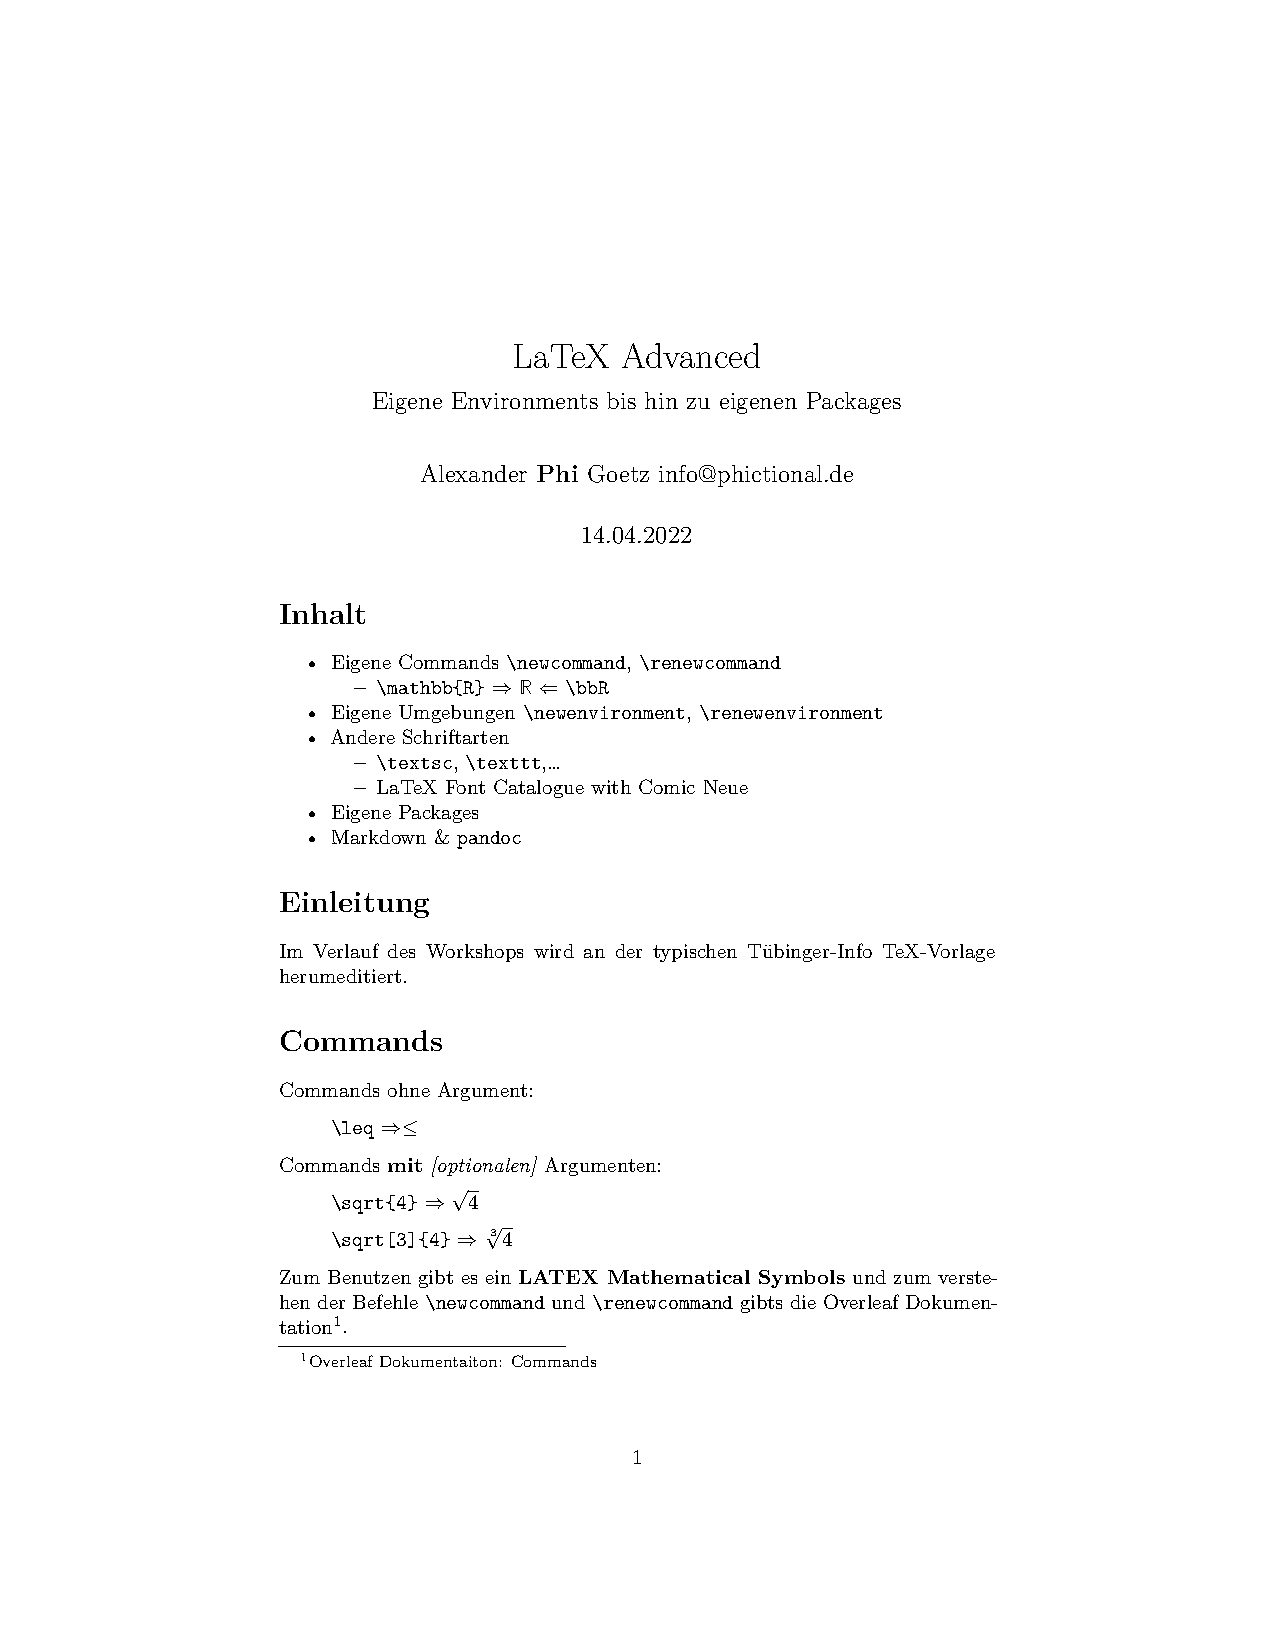
\includegraphics[page=1,height=1.2\textheight]{pictures/default.pdf}
        \end{figure}
    \end{columns}
\end{frame}

\begin{frame}[fragile]{\insertsection \quad\small Präsentationen}
    
    \begin{Beispiel}[\faMarkdown\faArrowRight\faTv\faFilePdf]
        \mint{sh}{>>> pandoc -f markdown -t beamer -o slides.pdf slides.md}
    \end{Beispiel}

    \begin{columns}
        \column{.47\linewidth}
        
        \begin{Beispiel}[\faMarkdown\faArrowRight\faTv HTML]
            \begin{minted}[fontsize=\small]{sh}
>>> pandoc \
>   -f markdown -t slidy \
>   -s --mathjax         \
>   -o slidy.html slides.md
            \end{minted}
        \end{Beispiel}
        
        
        \column{.005\linewidth}
        
        \column{.47\linewidth}
        
        \begin{Beispiel}[\faMarkdown\faArrowRight\faTv HTML]
            \begin{minted}[fontsize=\small]{sh}
>>> pandoc \
>   -f markdown -t revealjs \
>   -s --mathjax            \
>   -o revealjs.html slides.md
            \end{minted}
        \end{Beispiel}
        
    \end{columns}
\end{frame}


%-------------------------------------------------------------------------------
%       END ACTUAL CONTENT
%-------------------------------------------------------------------------------

\section*{Danke fürs mitmachen}
\begin{frame}
    \sectionpage
    \vspace{1em}
    \begin{columns}[c]
        \column{.7\textwidth}
        Wenn ihr uns mitteilen wollt, wie es euch gefallen hat:\\
        \faComment*[regular]\ \url{\linkFeedback}
        \column{.3\textwidth}
        \centering
        \qrcode[height=.6\textwidth]{\linkFeedback}
    \end{columns}
\end{frame}


\subsection*{Resourcen}
\newcommand{\linkitem}[2]{\item \textbf{#1}: \scriptsize\url{#2}\normalsize}
\begin{frame}{\insertsubsection}
    \begin{itemize}
        \linkitem{Material}{\linkMaterial}
        \linkitem{Font Catalogue}{\fontcalatogue}
        \linkitem{Font Awesome 5}{\ctanFontAwesome}
        \linkitem{Packages}{\overleafPackage}
        \linkitem{Classes}{\overleafClass}
        \linkitem{Package vs. Class}{\overleafPvC}
        \linkitem{Github Flavored Markdown Specification}{\gfmspec}
        \linkitem{Pandoc}{\pandoc} \scriptsize\quad\url{\pandocExamples}\normalsize
    \end{itemize}
\end{frame}


% \blankframe


\end{document} 
